\documentclass[11pt]{article}
\usepackage{UF_FRED_paper_style}

% \usepackage{natbib}
\usepackage{listings}
\usepackage{color}

\definecolor{dkgreen}{rgb}{0,0.6,0}
\definecolor{gray}{rgb}{0.5,0.5,0.5}
\definecolor{mauve}{rgb}{0.58,0,0.82}

\lstset{frame=tb,
  language= dafny,
  aboveskip=3mm,
  belowskip=3mm,
  showstringspaces=false,
  columns=flexible,
  basicstyle={\small\ttfamily},
  numbers=none,
  numberstyle=\tiny\color{gray},
  keywordstyle=\color{blue},
  commentstyle=\color{dkgreen},
  stringstyle=\color{mauve},
  breaklines=true,
  breakatwhitespace=true,
  tabsize=3
}

% \usepackage{lipsum} %% Package to create dummy text (comment or erase before start)
% \usepackage{subcaption}

\begin{document}
%% ===============================================
%% Setting the line spacing (3 options: only pick one)
% \doublespacing
% \singlespacing
\onehalfspacing
%% ===============================================

\setlength{\droptitle}{-5em} %% Don't touch

\begin{titlepage}
\newcommand{\HRule}{\rule{\linewidth}{0.1mm}} 
\center % Center everything on the page
 
%---------------------------------------------------------------------------------
%	HEADING SECTIONS (Enter the Homework/assignment No., only)
%---------------------------------------------------------------------------------

\textsc{\Large University of Waterloo}\\ % heading course Number
\textsc{\Large ECE653 - Softwart Test/Qual Assur/Maint}\\ % heading course name
\textsc{\large Project Report}\\ % Minor heading
%---------------------------------------------------------------------------------
%	TITLE SECTION (Replace 'TITLE' with the Homework/assignment Name/title)
%---------------------------------------------------------------------------------

\HRule \\[0.4cm]
{ \huge \bfseries Formal Verification of Solidity Smart Contracts Using Dafny }\\[0.1cm] % Title of your Homework/assignment
\HRule \\[1.5cm]
 
%---------------------------------------------------------------------------------
%	AUTHOR SECTION (EDIT THE NAME and T.NO., only)
%---------------------------------------------------------------------------------

\begin{minipage}{0.4\textwidth}
\begin{flushleft} \large

\emph{\bfseries Report by:}\\
Alireza \textsc{Lotfi Takami}\\
\emph{Student ID:} 20854299\\
\emph{Email:} alotfita@uwaterloo.ca
Krishna \textsc{Kantwala}\\
\emph{Student ID:} 20868348\\
\emph{Email:} kdkantwa@uwaterloo.ca
Aditi \textsc{Padade}\\
\emph{Student ID:} 20854299\\
\emph{Email:} aditi3049@gmail.com
\end{flushleft}

\end{minipage}
\begin{minipage}{0.4\textwidth}
\begin{flushright} \large
\emph{\bfseries Instructor:} \\
Dr. Vijay \textsc{Ganesh} % Supervisor's Name
\end{flushright}
\textsc{•}\textsc{•}\end{minipage}\\[2cm]
{\large \today}\\[1cm] 

\includegraphics[scale=.14]{figures/waterloo.png}% \\[0.5cm] % 
\vfill % Fill the rest of the page with white-space

\end{titlepage}

% %%%%%%%%%%%%%%%%%%%%%%%%%%%%%%%%%%%%%%%%%%%%%%%%%%%%%%%%%%
% %%%%%%%%%%%%%%%%%%%%%%%%%%%%%%%%%%%%%%%%%%%%%%%%%%%%%%%%%%
% BODY OF THE DOCUMENT
% %%%%%%%%%%%%%%%%%%%%%%%%%%%%%%%%%%%%%%%%%%%%%%%%%%%%%%%%%%
% %%%%%%%%%%%%%%%%%%%%%%%%%%%%%%%%%%%%%%%%%%%%%%%%%%%%%%%%%%

% --------------------
\section{Abstract}
% --------------------
\paragraph{}
A smart contract is a self-executing contract with the terms of the agreement between buyer and seller being directly written into lines of code. The code and the agreements contained therein exist across a distributed, decentralized blockchain network. The code controls the execution, and transactions are trackable and irreversible. Smart contracts permit trusted transactions and agreements to be carried out among disparate, anonymous parties without the need for a central authority, legal system, or external enforcement mechanism \cite{Website:1}. Solidity is a domain-specific programming language intended for smart contract development. It aims to reduce the transaction costs resulting from contract execution on distributed ledgers such as the Ethereum. 
\paragraph{}
Solidity contracts, however, must comply with safety and security standards, which require rigorous inspection and certification \cite{zhu2020formal}.This paper demonstrates the implementation of a verification tool to ensure bug-free designing of the smart contract . This tool is expected to take the smart contract written in solidity and translate it to dafny. Dafny being a static program verifier will be used to verify the functional correctness of the contract \cite{DafnyALa19:online}. We consider correctness as the state of the program without any bugs such that the program observes safe programming practices.

\section{Introduction}
\paragraph{}
A blockchain is a decentralised, distributed, and mostly public, digital ledger composed of records called blocks that are used to record transactions through various computers so that any block involved can not be retroactively changed without altering all subsequent blocks. This helps the participants to independently and fairly inexpensively review and inspect transactions. Using a peer-to - peer network and a distributed time stamping server, a blockchain database is managed autonomously They are authenticated by collective self-interest motivated by mass collaboration \cite{Blockcha25:online}. The biggest advantage of blockchain is that due to its decentralized nature of the network that operates between all the approved parties, there is no need to pay intermediaries \cite{WhatAreS98:online}.

\paragraph{}
Smart contracts are executable programs that enable
the building of a programmable trust mechanism between
multiple entities without the need of a trusted third-party. Smart contracts are often written in a Turing-complete programming language called Solidity, which is not easy to audit for subtle errors [see Abstract]\cite{Hardaker2004}. Although the faithful execution of a smart contract is enforced by the consensus protocol of the blockchain, it remains the prerogative of the participating organisations to check the validity of the smart contract , i.e., the syntactic implementation meets the best practises, and validate its fairness, i.e. the code adheres to the agreed higher-level business interaction logic.Although manual auditing of contracts is possible to some degree for accuracy, it still remains laborious and vulnerable to error. In comparison, automated formal auditing requires professional resources and reasoning. The problem gets worse with the the fact that, unlike other distributed system code, smart contracts are permanent and hard to fix in the case of bugs, regardless of how much money they possess \cite{kalra2018zeus}.

\paragraph{}
Therefore, to ensure bug-free smart contract we propose command-line a tool which will verify the smart contract using static verification. Since Smart contracts are coded in an object- oriented programming language called Solidity which does not support static verification, there was a requirement of another programming language in which the smart contracts will be translated and the translated code shall be verified for the potential bugs. This requirement shall be fulfilled by Dafny which supports formal verification.

%------------------------
\section{Our Method}
%------------------------
\paragraph{}
As we know ensuring that a smart contract is correct is very important because now days considerable amount of money is controlled by blockchains and smart contracts. Therefore, we can say that smart contracts are a kind of safety-critical systems. As smart contracts failure leads to catastrophic consequences, it is very important to do formal verification on them before deploying them on blockchains. Doing smart contracts verification manually is too time consuming and most of the smart contract developers do not have enough knowledge and expertise in software testing and formal verification. Therefore, creating a tool that do this formal verification automatically could be very beneficial. 
\paragraph{}
In this project we are going to propose a solidity static verification tool. To do this verification on smart contract functions we need to add some queries to the smart contract solidity code and then verify that if the smart contract function satisfies the provided queries or not. 
\paragraph{}
In order to implement the Smart contract verification tool we need to turn smart contract into a state machine or another programming language that have the capability to apply static verification. Hence, we need a tool to parse solidity code and then turn int into our target language or state machine. Here we are going to use ANTLR which will help us to turn the input solidity code into a parse tree in a specific target language like Java or python.
\paragraph{}
In order to apply the static verification we decided to turn the solidity code into Dafny code. Dafny being a supporter of formal verification tool which will verify the translated code, thus giving an output in the form of a report with a list of detected error, if any. We used Python as target language of ANTLR parse tree to turn the parse tree into Dafny code. In general the input of our Solidity smart contract verification tool is a solidity smart contract function and its output is an equivalent Dafny code which then we can add some queries to it to do static verification on it. In the following section we are going to in detail explain the tool chain that we have used in this project to implement the solidity smart contract verification tool. 

%------------------------
\section{Tool Chain}
%------------------------
\paragraph{}
We have used different tools in our project to correctly verify smart contracts. In this section we are going to explain each of the tool which briefly focus on writing contracts in solidity, parse it through the antlr and verify the contracts with some description of the design of Dafny.

\subsection{Smart contracts}
\paragraph{}
Smart contracts are the building blocks that are used to create decentralized application.

\subsection{Solidity}
\paragraph{}
Solidity is a programming language which is used for implementing smart contracts. With the help of Solidity, we can write applications that implement self-enforcing business logic such as voting, crowdfunding, blind auctions, and multi-signature wallets. Even we can say that solidity is smart contract specific language\cite{Solidity82:online}. Smart contracts which are implemented in solidity language are self-executing piece of code that are compiled and pushed to the Ethereum blockchain for the execution without requiring centralized or trusted parties. Solidity program is complied to bytecode that is executable on the EVM (Ethereum virtual machine). EVM  is basically a runtime environment for smart contracts in Ethereum.
\paragraph{}
Solidity is a contract specific object-oriented programming language where each contract can have features like objects in OOPS such as common data types, state variables, functions and a contract-specific features including event notifiers, global variables, and modifier clauses of the contract \cite{Introduc89:online}. Consider the simple contract given below: \\
\begin{lstlisting}
pragma solidity ^0.5.0;

contract MyFirstContract {
    uint balance;
    
    function set(unit x) public {
        balance = x;
    }
    
    function get() public view returns (unit){
        return balance;
    }
}
\end{lstlisting}
As shown in the above code example, any solidity code file ought to begin with a "version pragma" for the code to use, which is the declaration of the version of the solidity compiler. It helps to prevent problems with future compiler versions where code with existing version could behave differently. \\

Contract can be created with the keyword contract and name of the .sol file. A contract is the basic building unit of Ethereum’s decentralized applications where all the methods and variables are the part of the contract. In this example, the contract declares a state variable balance of the unsigned integer of 256 bits and defines the methods set and get that can fetch and update the value of the variable. The solidity compiler then takes this high-level code, breaks it down in simple instructions, and convert it into byte code that is executable on the EVM.

\subsection{Antlr}
\paragraph{}
Antlr (Another Tool for Language Recognition) is a powerful parser generator, a tool which helps to create parser for reading, processing, executing or translating structured text or binary files. To parse a typical program using regular expression is not enough specially when program is using recursion but with the help of Antlr it becomes easier, faster and mess free. 
\paragraph{}
Antlr is used to build languages, tools, and frameworks. With the help of Antlr, one can generate a parser that can build and walk parse trees in their specific target language. Antlr helps to define a grammar for the language, data format, diagram or any kind of structure that is represented with text for analyzing \cite{ANTLR17:online}.
\paragraph{}
To deeply studying parser we need to initially focus on the lexers also known as tokenizers that take the separate characters and build the logical structure by transforming them into tokens. Antlr uses the grammar to generates code that describes what is legitimate in the language and how the language is structured and convert this grammar file into two parts: parser and lexer. A lexer reads the input stream and turns into tokens and parser associates the tokens with the elements of the grammar.
\paragraph{}
We have used solidity parser for python which built on the ANTLR 4 grammar file for the solidity programming language which helped to generate the solidity parse tree based on the given contract and grammar file in python and allows us to write code that handles the events from the parser.

\subsubsection{Dafny}
\paragraph{}
Dafny is an imperative object-oriented programming language which is used to verify the functional correctness of programs with the help of built-in automatic program verifier. Dafny is using built-in specification construct to support formal verification of program. These specifications include preconditions, post-condition, frame specifications, termination metrics, loop variants and loop invariant which helps to prove correctness of code \cite{DafnyALa66:online}. With the help of Dafny, it becomes easier for programmers to write correct code without having any run time errors and also correct in terms of what specifically program supposed to do. 
\paragraph{}
Dafny allows to write verifiable programs that automatically check the correctness of the smart contracts. To prove the correctness of the code Dafny depends on high-level annotations. The result of a chunk of code may be given abstractly which is less complicated and less error vulnerable to write. Dafny generates a proof that the code matches the annotations and lighten the load of writing bug-free code \cite{rise4fun9:online}". As the annotations are shorter and more direct it becomes easier to write code. Main concepts of the Dafny are described here.\\ \\
\textbf{Method: }
\paragraph{}
For any Dafny programs, one of the basic units is the "method" which is piece of executable code. Consider the following example: \\
\begin{lstlisting}
method addSub(a:int, b:int) returns (addition:int,subtraction:int)
{
    addition := a + b;
    subtraction := a - b;
    return addition, subtraction;
}
\end{lstlisting}
This code declares a method to perform addition and subtraction functionality which takes two integer parameter called "a" and "b" as an input and returns results "addition" and "subtraction" in integer. The code for the body of the method contained within the braces can consists of a series of statements including conditions, loops, method calls, return etc. Our method body calculating the addition and subtraction for the given input parameters and returning the result.
\\ \\
\textbf{Pre and post conditions: }
\paragraph{}
To specify the behavior of the methods, here comes the power of Dafny with annotations. Pre and Postconditions have their own keywords "requires" and "ensures" respectively and can be given as part of the method's declaration. Let's say for the above code example, any non-negative integer addition will always greater than subtraction. To implement this we can add annotations as given below: \\
\begin{lstlisting}
method addSub(a:int, b:int) returns (addition:int,subtraction:int)
    requires a > 0
    requires b > 0
    ensures addition > subtraction
{
    ....
}
\end{lstlisting}
Dafny verifies the code as correct with the help of these conditions because this assumption is enough to ensure that the code in the method body is correct.\\ \\
\textbf{Assert: }
\paragraph{}
Assertions declared with the assert statement for testing, debugging or proof purposes which says that a particular expression always holds when control reaches that part of the code. Whenever the Dafny encounters an assertion, it tries to prove that conditions hold for all executions of the code. \\
\begin{lstlisting}
method testing()
{
    var a:= 20;
    var b:= 10;
    var add,sub := addSub(a,b);
    assert add > sub;
}
\end{lstlisting}
In the above example, Dafny is able to prove the annotation easily for the method addSub as it is similar to the post-condition given in the method declaration.
\paragraph{}
Overall, examining the pre and post condition and writing assertions to verify assumptions in Dafny can guarantees that existing code is not broken. To understand more detail version of Dafny can be found at \cite{rise4fun9:online}.


%------------------------
\section{Results}
\paragraph{}
In order to evaluate our approach we have created ten solidity smart contracts. We used these ten smart contract as inputs of our Solidity smart contract formal verification tool. The Solidity formal verification tool then turns the solidity functions into Dafny functions. Hence, The ouptut of our tool is a Dafny function code. Then we can use Dafny code syntax to add queries to to Dafny function and verifiy different variables and parameters of the smart contract function. In the subsequent two sections we are going to explain how this tool have been implemented and we also show some input solidity functions and their equivalent Dafny function with verification queries. 

\subsection{Experimental Setup}
\paragraph{}
As we explained in last sections, in order to implement the solidity smart contract formal verification tool, we used Antlr, Python, and Dafny. Antler uses an input code and its proper grammar as its inputs and creates a parse tree which can be used for any purpose.  In the solidity smart contract verification project we feed Antlr with smart contract solidity code and a proper grammar file. We did not apply any changes on the input grammar file but in future to add more features to the project and make it more flexible we have to apply some changes on the solidity grammar file. So, in our case the output of Antlr is a solidity parse tree. Antlr has the option to create the parse tree for some different darget languages like Python and Java. Figure \ref{fig:parstree} indicates created parse tree for a simple input solidity function which only contains a return statement.
\begin{figure}[h]
    \centering
    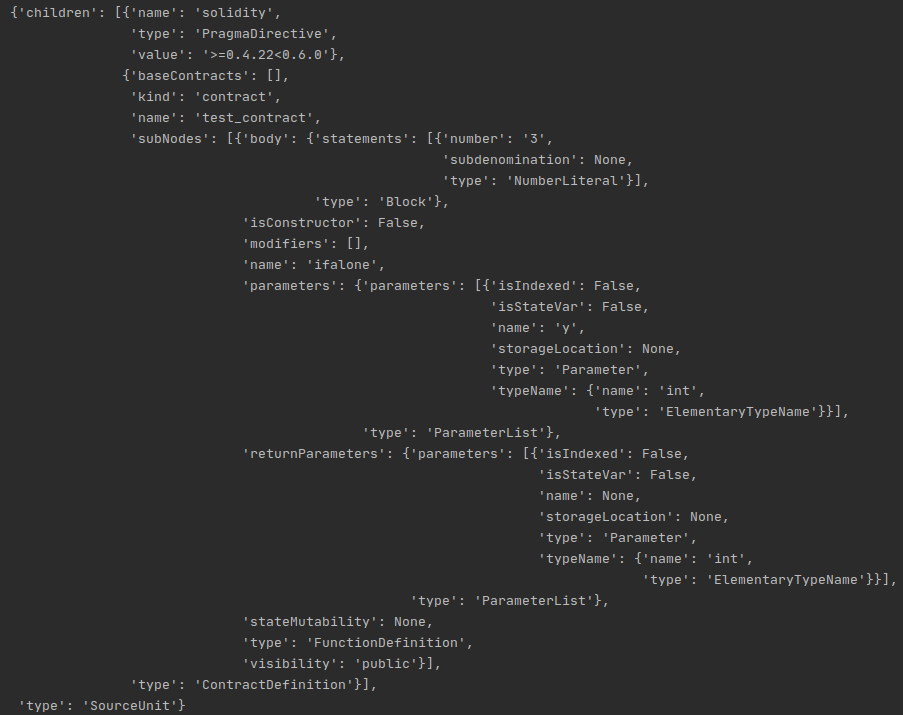
\includegraphics[width=0.9\textwidth]{figures/parsetree.png}
    \caption{Parse tree of a simple solidity function with only one return statement.}
    \label{fig:parstree}
\end{figure}
\paragraph{}
As Python decreases the development time, we used python as Antlre target language. Therefore, in our project the parse tree of Antlre can be used by Python. We used Python to use Antlre's output parse tree and also to create a command-line user interface as interface of our solidity smart contract formal verification tool. As covering all solidity syntax is a time consuming task, we started by solidity basic syntax and turned the solidity parse tree into Dafny code. In next step we added some verification queries to the Dafny code and Then checked to see weather this quires will be satisfied or not. In section \ref{ER} we are going to provide the experimental results which are some inputs and outputs of our solidity smart contract formal verification tool.

\subsection{Experimental Results}\label{ER}
\paragraph{}
We test the solidity smart contract verification tool using ten different input solidity codes. From the experimental results it can be seen the implemented tool and proposed solidity smart contract verification approach can correctly be used for smart contract verification. As we said we used ten different smart contracts solidity code to check correctness of our approach but here were are going to show two different input solidity smart contracts and their output which were produced by our solidity smart contract verification tool. 

\paragraph{}
Figure \ref{fig:res1} shows a solidity smart contract and its equivalent Dafny code which has been produced by our solidity smart contract verification tool. Where Figure \ref{fig:res1fig1} show the solidity smart contract function which consist of one if-else statement. We used this solidity code as input to our solidity smart contract verification tool. The equivalent Dafny code of the solidity code is Figure \ref{fig:res1fig2} which has been produced by our Solidity verification tool. After producing the Dafny code, we added some queries to it to do the verification. For example we have added a "require" and an "assert" statement to the produced Dafny code. We can add any other queries using Dafny syntax to verify any variables in the solidity code. 

\begin{figure}
\begin{subfigure}{.52\textwidth}
  \centering
  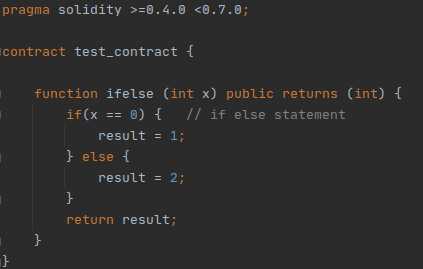
\includegraphics[width=.8\linewidth]{figures/ifelse_sol.png}
  \caption{Solidity code}
  \label{fig:res1fig1}
\end{subfigure}%
\begin{subfigure}{.48\textwidth}
  \centering
  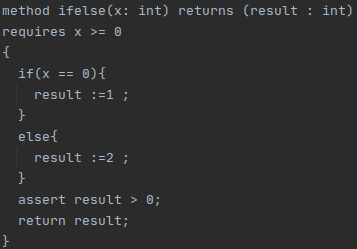
\includegraphics[width=.8\linewidth]{figures/ifels_dfy.png}
  \caption{Dafny code}
  \label{fig:res1fig2}
\end{subfigure}
\caption{Verification of a solidity smart contract function with one if-else statement.}
\label{fig:res1}
\end{figure}

\paragraph{}
Figure \ref{fig:res2} shows another solidity smart contract and its equivalent Dafny code which has been produced by our solidity smart contract verification tool. Where Figure \ref{fig:res2fig1} show the solidity smart contract function which consist of a nested if-else statement. We used this solidity code as input to our solidity smart contract verification tool. The equivalent Dafny code of the solidity code is Figure \ref{fig:res2fig2} which has been produced by our Solidity verification tool. After producing the Dafny code, we added some queries to it to do the verification. For example we have added an "ensures" and a "require" statement to the produced Dafny code. We can add any other queries using Dafny syntax to verify any variables in the solidity code. With the same way we have created 8 other solidity smart contract and we verified them using their equivalent Dafny code which were produced by our verification tool.

\begin{figure}
\begin{subfigure}{.50\textwidth}
  \centering
  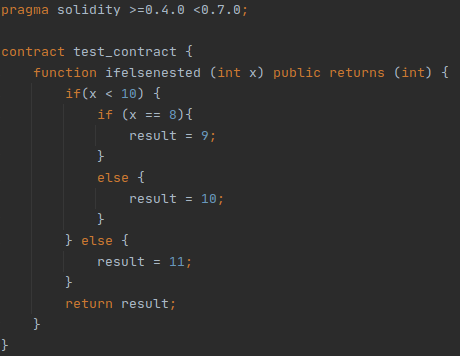
\includegraphics[width=.8\linewidth]{figures/ifelsenested_sol.png}
  \caption{Solidity code}
  \label{fig:res2fig1}
\end{subfigure}%
\begin{subfigure}{.48\textwidth}
  \centering
  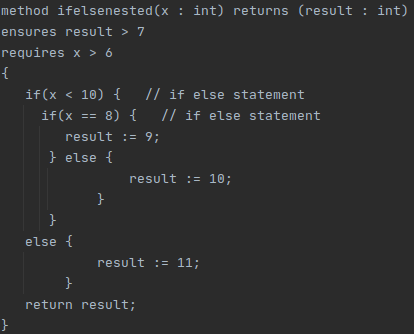
\includegraphics[width=.8\linewidth]{figures/ifelsenested_dfy.png}
  \caption{Dafny Code}
  \label{fig:res2fig2}
\end{subfigure}
\caption{Verification of a solidity smart contract function with nested if-else statement.}
\label{fig:res2}
\end{figure}


\section{Future Work}
\paragraph{}
As we explained, we started the solidity smart contract verification tool by covering some basic syntax of solidity. In the next step, we need to cover all solidity syntax. Then we can turn any arbitrary smart contract functions into its equivalent Dafny code. Therefore we can verify all smart contracts. Another feature that need to be added to the verification tool is adding query syntax directly to Solidity code. In this way, The smart contract developer does not need to know anything about Dafny and the Dafny queries could be easily added directly to the smart contract code. 

% \medskip


\bibliography{references} 


\end{document}


